\documentclass{standalone}

\usepackage{tikz}
\usetikzlibrary{positioning, calc}

% new command: interval
\newcommand{\itv}[5] % #1: start point; #2: end point; #3: interval name; #4: operation; #5: color 
{
  \coordinate (start #3) at #1;	% start point
  \coordinate (end #3) at #2;	% end point
  \coordinate (mid) at ($0.5*#1 + 0.5*#2 + (0,0.3cm)$);
  \node [font = \large] at (mid) {\texttt{#4}};	% attach the operation 
  \draw[ultra thick, #5, |-|] (start #3) -- (end #3) node (#3) {}; % draw the interval and give it a name 
}

\begin{document}
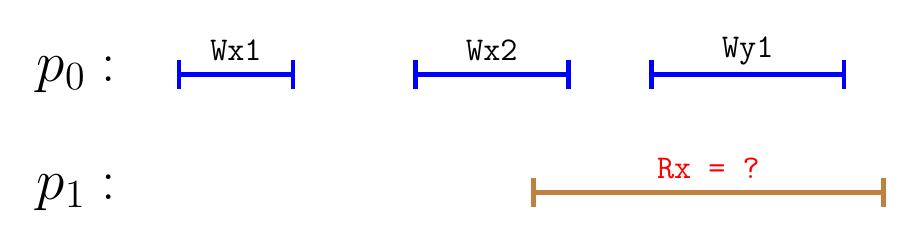
\begin{tikzpicture}
  \itv{(0,0)}{(1.5,0)}{wx1}{Wx1}{blue}
  \itv{(3,0)}{(5.0,0)}{wx2}{Wx2}{blue}
  \itv{(6,0)}{(8.5,0)}{wy1}{Wy1}{blue}
  \itv{(4.5,-1.5)}{(9.0,-1.5)}{rx}{}{brown}

  % client processes
  \node (p0) [left = 2.0cm of wx1.west, font = \huge] {$p_0:$};
  \draw let \p{p0} = (p0), \p{rx} = (rx) in 
    node (p1) [font = \huge] at (\x{p0}, \y{rx}) {$p_1:$};

  % a dirty trick to reuse "mid" of the last interval
 \node () [font = \large, red] at (mid) {\texttt{Rx = ?}};	% attach the operation name  
\end{tikzpicture}
\end{document}
